\chapter{Square cylinder}
The square cylinder problem studies the two-dimensional laminar flow around a square cylinder inside a plane channel. The description of the problem can be seen in figure \ref{SchemeSquareProblem}.
\begin{figure}[h]
	\centering
	\includegraphics[scale=0.5]{Square/Definition}
	\caption[General scheme of the square cylinder problem]{General scheme of the square cylinder problem. Extracted from \cite{Breuer2000}}
	\label{SchemeSquareProblem}
\end{figure}

\section{Discretization}
In this kind of problem, the region near the cylinder has an important pressure and velocity gradient whereas in the rest of the channel flow they are smoother. So, near the cylinder a finer mesh is needed, but not in the whole domain of the problem. Using a very fine mesh in all the channel would be computationally expensive and inefficient, but a coarser mesh would lead to inaccurate results, especially in the cylinder.

The domain is divided in three parts, vertically and horizontally. The mesh that contains the obstacle is a uniform mesh of very high precision, whereas the other meshes are also uniform but coarser. The details of the discretization are in table \ref{NumericalCylinder}.
\begin{table}[h]
	\centering
	\begin{tabular}{ |c|c|c|c|c|c|c|c|c|c|c|c|c| }
		\hline
		$N_{1}$ & $N_{2}$ & $N_{3}$ & $M_{1}$ & $M_{2}$ & $M_{3}$ & $D$ & $H$ & $L$ & $l$ & $\rho$ & $u_{max}$ & $\delta$ \\ \hline
		$90$ & $10$ & $300$ & $30$ & $10$ & $30$ & $1$ & $8D$ & $50D$ & $L/4$ & $1$ & $1$ & $10^{-4}$ \\ \hline
	\end{tabular}
\caption{Numerical parameters of the square cylinder problem}
\label{NumericalCylinder}
\end{table}


\section{Boundary conditions}
\subsection{Inlet conditions}
Since the flow is inside a channel, the inflow has a parabolic velocity profile with a maximum velocity $u_{max}$ in the centre:
\begin{equation}
u\left(y\right)=4u_{max}\left[\left(\frac{y}{H}\right)-\left(\frac{y}{H}\right)^{2}\right]
\end{equation}
This maximum velocity defines the Reynolds number of the problem:
\begin{equation}
Re=Re_{max}=\frac{\rho u_{max}D}{\mu}
\end{equation}
As for the pressure conditions, a Neumann condition is imposed:
\begin{equation}
\frac{\partial p}{\partial x}=0
\end{equation}

\subsection{Outlet conditions}
In order to have a developed flow in the outlet, it is important to have a distance large enough between the position of the cylinder and the end of the channel in order to have fully developed flow. To define the outflow, a convective boundary condition is used:
\begin{equation}
\frac{\partial u}{\partial t}+u_{conv}\frac{\partial u}{\partial x}=0
\end{equation}
where $u_{conv}$ is equal to the maximum velocity $u_{max}$ of the parabolic inflow velocity profile. The integration over time of this condition is done using an Adams-Bashforth scheme.

In the outlet, as opposite to the inlet, a Dirichlet condition is used to determine the pressure:
\begin{equation}
p=0
\end{equation}

\subsection{Wall conditions}
In the channel walls the no-slip condition is applied:
\begin{equation}
\vec{v}=0
\label{noslip}
\end{equation}
As well as the boundary layer condition, in which the pressure gradient normal to the wall is 0.

In the convection problems studied in the previous sections the flow was developing inside a cavity with no other obstacles than the walls. In this problem, the fluid flows around a square cylinder, so the boundary conditions have to be also implemented for the cylinder. Since it is a solid object and it does not allow air to flow through it, it is treated as a wall \cite{Ferziger2002}. Consequently the velocity in its boundary is also given by equation \ref{noslip}.

\section{Algorithm}
The algorithm used in the resolution of this problem is the same used in the calculation of the driven cavity problem (section \ref{AlgorithmDriven}).

\section{Results}
Depending on the Reynolds number the wake of the cylinder is completely different. In the following results, the fluid is only studied for $1\leq Re<60$, the steady regime. For $Re\geq60$ the fluid changes completely its behaviour and never reaches a steady state. It is called the unsteady regime.

Figure \ref{HorizontalCylinder} shows the distribution of the horizontal velocity as a function of the Reynolds number. When the fluid reaches the cylinder it slows down, but when it is passing it the flow accelerates. In the rear side of the cylinder there is a zone with negative velocity. As the Re increases the accelerated area and the zone with reverse flow increase as well. Regarding the general distribution of velocities, for low Re it is almost symmetric, but as the Re increases it stretches to the right.

Regarding the vertical velocity (figure \ref{VerticalCylinder}), in order to avoid the cylinder, the flow moves up near its upper edge and down near the lower edge. In the rear side of the cylinder the movement is completely the opposite. Again, for low Re the distribution is more or less symmetric, but as the Re increases it stretches to the right and the gradient of velocities in the frontal edges of the cylinder increases as well.

Finally, the fluid flow is completely defined by the streamlines of figure \ref{StreamlinesCylinder}. At $Re=1$ the flow passes the cylinder without separation. But passed $Re\approx5$, two symmetric vortices appear in the rear side of the cylinder. The length of these vortices increases with the Reynolds number.

In conclusion, for low Re, viscosity avoids the separation of the laminar boundary layers. But as the Re increases and convection becomes more important there is a separation of the boundary layer in the rear side of the cylinder that generates the obtained symmetrical vortices.

\begin{figure}[h!]
	\centering
	\begin{subfigure}{0.5\textwidth}
		\resizebox{1.1\textwidth}{!}{\input{Square/u1}}
		\caption{$Re=1$}
	\end{subfigure}%
	\begin{subfigure}{0.5\textwidth}
		\resizebox{1.1\textwidth}{!}{\input{Square/u3}}
		\caption{$Re=3$}
	\end{subfigure}
	\begin{subfigure}{0.5\textwidth}
		\resizebox{1.1\textwidth}{!}{\input{Square/u5}}
		\caption{$Re=5$}
	\end{subfigure}%
	\begin{subfigure}{0.5\textwidth}
		\resizebox{1.1\textwidth}{!}{\input{Square/u10}}
		\caption{$Re=10$}
	\end{subfigure}
	\begin{subfigure}{0.5\textwidth}
		\resizebox{1.1\textwidth}{!}{\input{Square/u30}}
		\caption{$Re=30$}
	\end{subfigure}%
	\begin{subfigure}{0.5\textwidth}
		\resizebox{1.1\textwidth}{!}{\input{Square/u50}}
		\caption{$Re=50$}
	\end{subfigure}
\caption{Horizontal velocity near the cylinder}
\label{HorizontalCylinder}
\end{figure}

\begin{figure}[H]
	\centering
	\begin{subfigure}{0.5\textwidth}
		\resizebox{1.1\textwidth}{!}{\input{Square/v1}}
		\caption{$Re=1$}
	\end{subfigure}%
	\begin{subfigure}{0.5\textwidth}
		\resizebox{1.1\textwidth}{!}{\input{Square/v3}}
		\caption{$Re=3$}
	\end{subfigure}
	\begin{subfigure}{0.5\textwidth}
		\resizebox{1.1\textwidth}{!}{\input{Square/v5}}
		\caption{$Re=5$}
	\end{subfigure}%
	\begin{subfigure}{0.5\textwidth}
		\resizebox{1.1\textwidth}{!}{\input{Square/v10}}
		\caption{$Re=10$}
	\end{subfigure}
	\begin{subfigure}{0.5\textwidth}
		\resizebox{1.1\textwidth}{!}{\input{Square/v30}}
		\caption{$Re=30$}
	\end{subfigure}%
	\begin{subfigure}{0.5\textwidth}
		\resizebox{1.1\textwidth}{!}{\input{Square/v50}}
		\caption{$Re=50$}
	\end{subfigure}
	\caption{Vertical velocity near the cylinder}
	\label{VerticalCylinder}
\end{figure}

\pagebreak
\begin{figure}[H]
	\centering
	\begin{subfigure}{0.5\textwidth}
		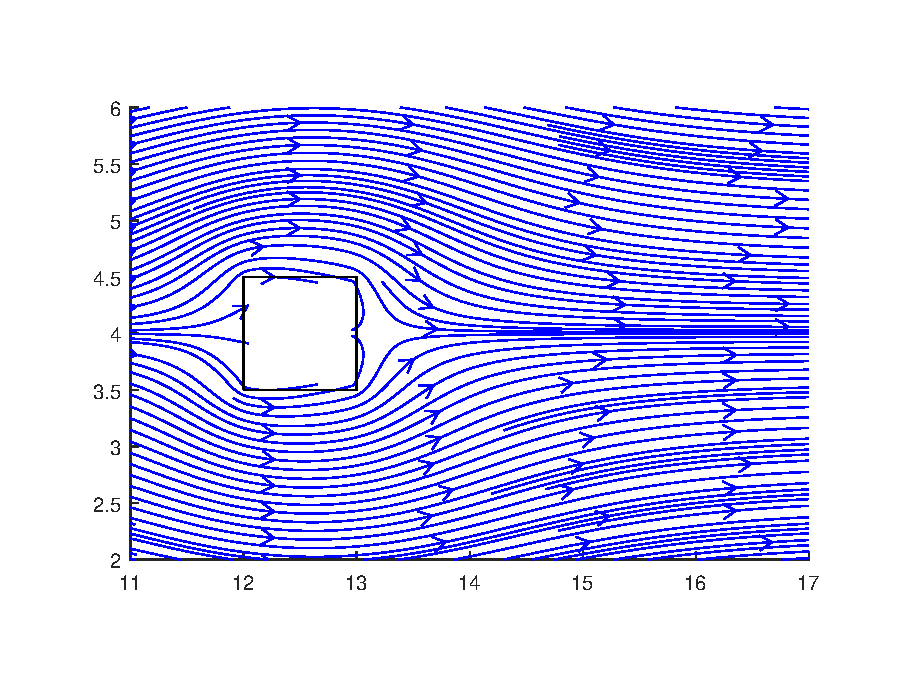
\includegraphics[scale=0.6]{Square/1}
		\caption{$Re=1$}
	\end{subfigure}%
	\begin{subfigure}{0.5\textwidth}
		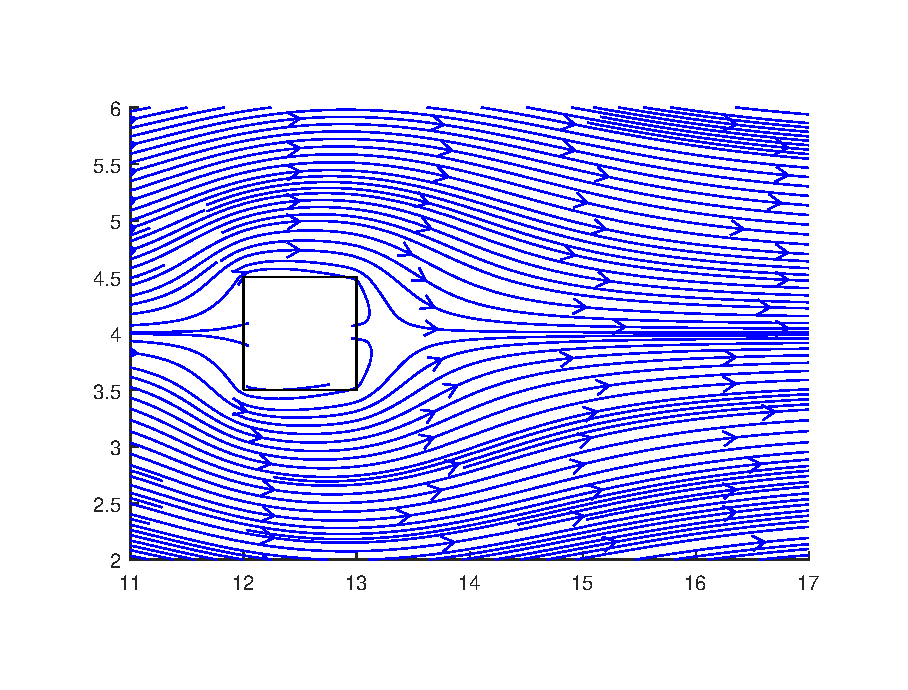
\includegraphics[scale=0.6]{Square/3}
		\caption{$Re=3$}
	\end{subfigure}
	\begin{subfigure}{0.5\textwidth}
		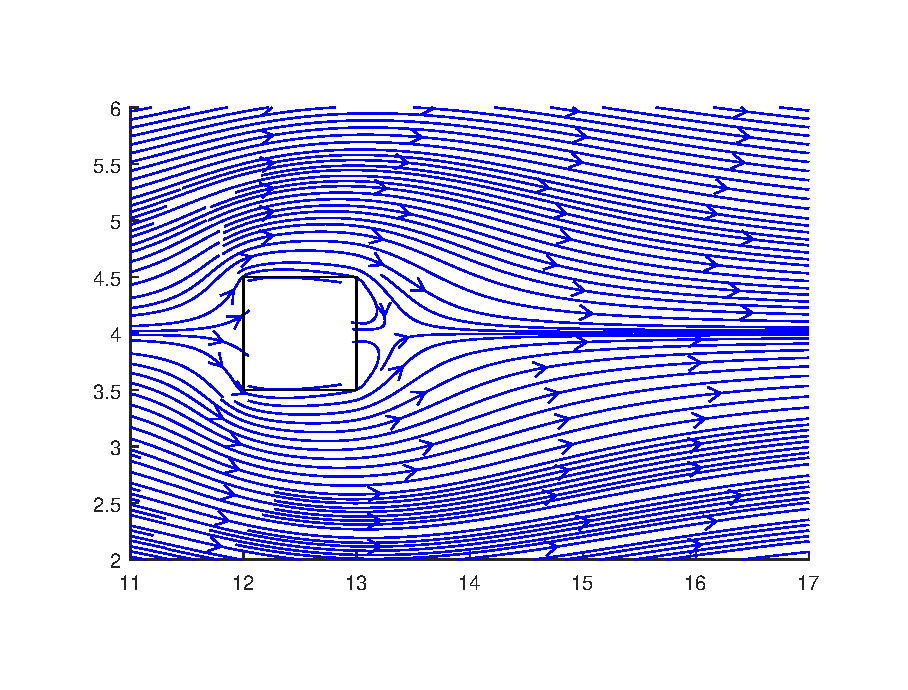
\includegraphics[scale=0.6]{Square/5}
		\caption{$Re=5$}
	\end{subfigure}%
	\begin{subfigure}{0.5\textwidth}
		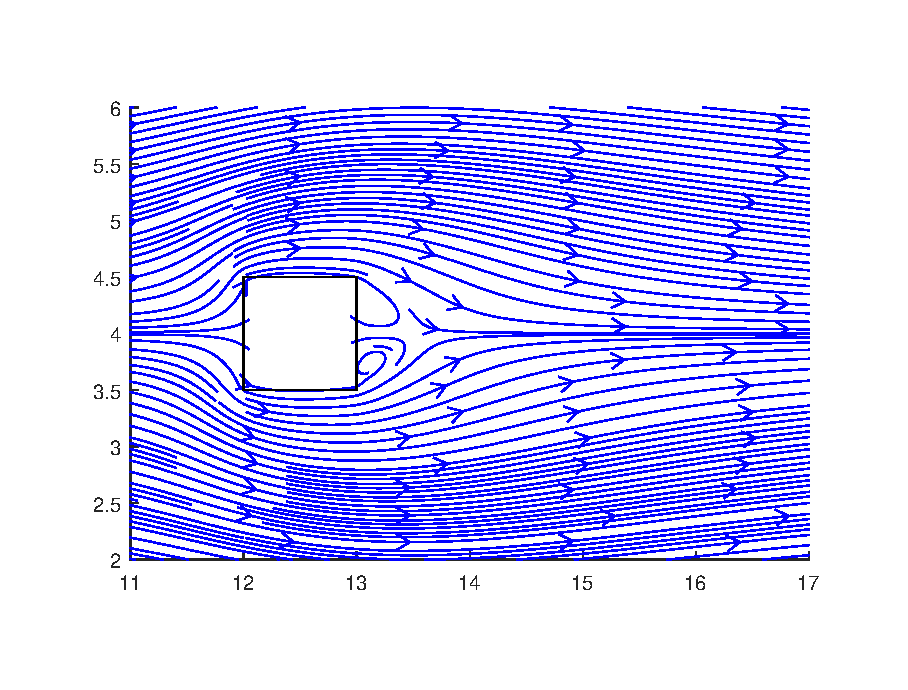
\includegraphics[scale=0.6]{Square/10}
		\caption{$Re=10$}
	\end{subfigure}
	\begin{subfigure}{0.5\textwidth}
		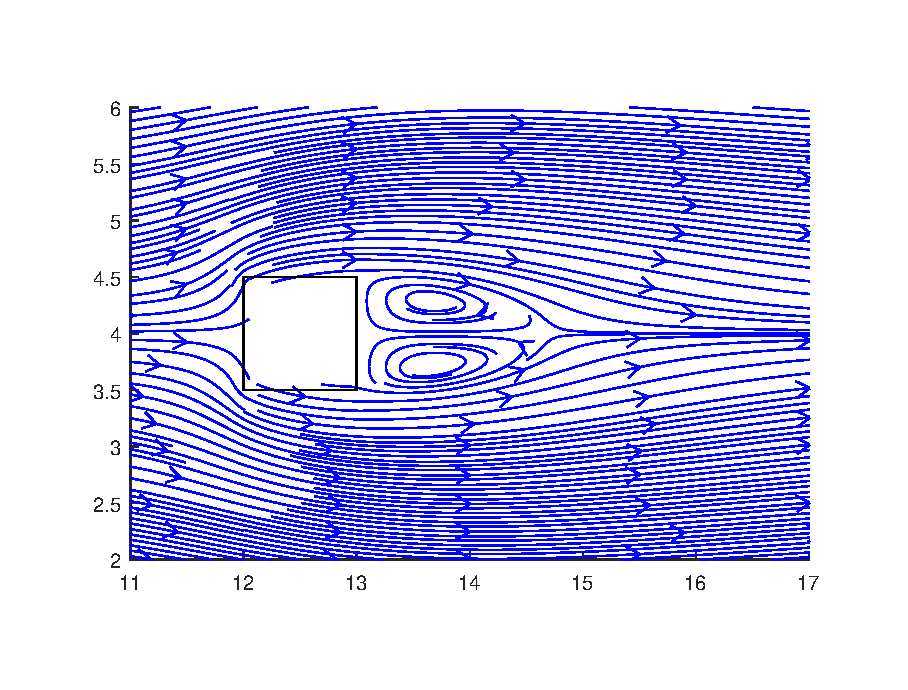
\includegraphics[scale=0.6]{Square/30}
		\caption{$Re=30$}
	\end{subfigure}%
	\begin{subfigure}{0.5\textwidth}
		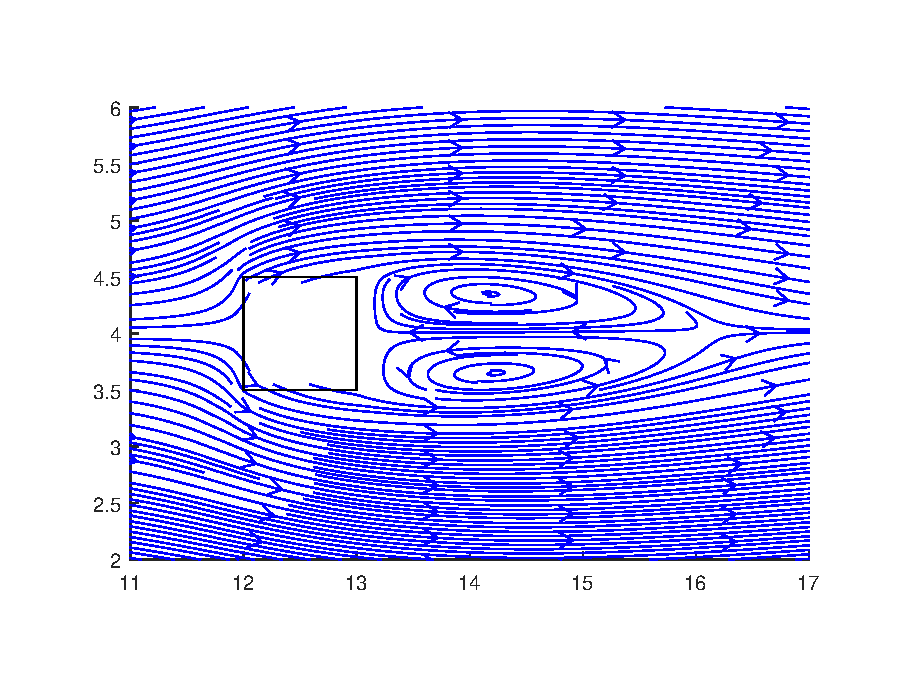
\includegraphics[scale=0.61]{Square/50}
		\caption{$Re=50$}
	\end{subfigure}
	\caption{Vertical velocity near the cylinder}
	\label{StreamlinesCylinder}
\end{figure}

\pagebreak
An important parameter of the problems that study the flow around an object is the length of the closed wake behind the cylinder. According to \cite{Breuer2000}, the recirculation length has a linear dependence on the Reynolds number:
\begin{equation}
L_{r}/D=-0.065+0.0554Re \quad \textrm{for} \quad 5<Re<60
\end{equation}

The recirculation length is obtained comparing the horizontal velocities of the central horizontal plane. In the wake the velocity is negative, but in the external flow the velocity is positive. The recirculation length is the distance between the rear side of the cylinder and the point in which the velocity changes from negative to positive.

Figure \ref{RecirculationReynolds} compares the calculated results with the reference ones as a function of the Reynolds number. The results are very similar, but at low Re the error is quite high. It could be due to the mesh. At low Re the recirculation length is very small, so it can only be accurately measured with a very fine mesh.
\begin{figure}[H]
	\centering
	\input{Square/Recirculation}
	\caption{Recirculation length vs. Reynolds number}
	\label{RecirculationReynolds}
\end{figure}